\documentclass[11pt]{article}
\usepackage[utf8]{inputenc}
\usepackage[T1]{fontenc}

\usepackage{mathptmx}

\usepackage[]{geometry}
\usepackage{listings}
\usepackage{natbib}
\usepackage{graphicx}
\usepackage{url}
\usepackage{xcolor}
\usepackage[parfill]{parskip}
\lstset{basicstyle=\footnotesize\ttfamily,breaklines=true}

\title{Analysing Orphaned Triples in a Large-Scale Graph Database}
\author{Gary Gurlaskie}
\date{15 April 2020}

\begin{document}

\begin{titlepage}
 \centering
 \vspace*{1in}
 \begin{Large}\bfseries
  Analyzing Orphaned Triples in a Large-Scale Graph Database\par
 \end{Large}

 \vspace*{0.2in}

  CIS4914 -- Final Report\par
  Spring 2020\par

  \vspace*{0.2in}
  
  Gary Gurlaskie (\url{g.gurlask@ufl.edu})\par
  Individual Project\par
  16 April 2020\par
\end{titlepage}

\section*{Abstract}
This project emphasized data analysis and visualization, and was focused on UF VIVO, a 7.1GB RDF graph database that documents UF research efforts. The goal was to identify data in VIVO that had become "orphaned" (disconnected) from the graph.

The analysis was performed ad hoc using Python. Analysis performed included examining zero- or low-degree nodes, connected components, and performing constraint validation against the published ontology.

The work yielded over 10,000 orphaned triples. However, the quality of the data was high overall; 94\% of the graph was connected robustly.

\section*{Introduction}
This project was focused on the analysis and visualization of orphaned data in UF VIVO, a 7.1GB graph database that documents UF research efforts. The database is managed by the UF Clinical and Translational Science IT (CTS-IT) and the VIVO application is publicly accessible at \url{vivo.ufl.edu}. This project was selected because it involved working with real-world data on a large scale. This data has been managed by the CTS-IT for years, and they have several full- and part-time employees working on the development of the VIVO application. Moreover, this project has a positive impact on data quality (and potentially database performance) for the University of Florida, which makes it desirable to complete as well.

The project mainly involved the application of basic database and graph algorithms (i.e., table scan, indexing, union-find) to an RDF database, so the majority of the literature surveyed relates to the RDF database itself. RDF databases are essentially composed of a list of "triples" [RDF]. The triples are values of the form "subject, predicate, object", where each element is a URI. These values carry semantic meaning -- for example, one triple might be "entity-n9633259703 has-type person", or more concretely:

<http://vivo.ufl.edu/individual/n9633259703> <http://www.w3.org/1999/02/22-rdf-syntax-ns\#type> <http://xmlns.com/foaf/0.1/Person>

The UF VIVO database also carries an "ontology". The ontology introduces both constraints and an inheritance structure on the triples [OWL]. Readers familiar with object-oriented programming may find this similar to the Java programming language. Different ontologies are typically combined to form the "schema" for the composite database -- for example, the VIVO ontology uses the FOAF ("friend of a friend"), OBO ("Open Biological and Biomedical Ontology") and VCARD ontologies. The VIVO ontology also introduces classes such as "vivo:Authorship", which relates a "foaf:Agent" and an "obo:InformationContentEntity" (a generic class whose subclasses include "bibo:article" or "obo:TextualEntity"). Relations like "vivo:Authorship" can carry additional metadata, such as dates and labels. "vivo:Authorship" also carries constraints, such as that it must include at least one "vivo:relates" edge to a "foaf:Agent" and at least one "vivo:relates" edge to an "obo:InformationContentEntity" [OWL]. A subset of the VIVO ontology is depicted in Figure 1.

\begin{figure}[h!]
\centering
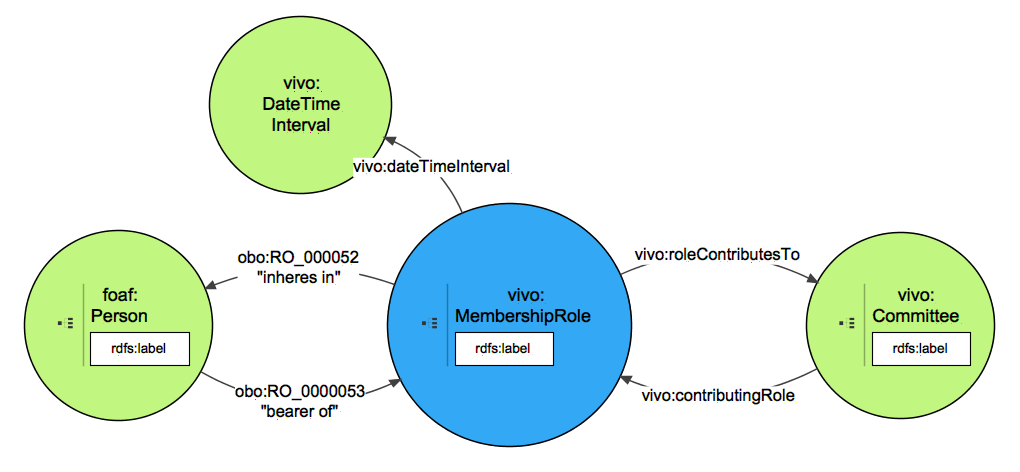
\includegraphics[width=11cm]{membership-model.png}
\caption{VIVO committee model [VIVO] (CC BY 4.0, cropped)}
\label{fig:output}
\end{figure}

The data analyzed was in N-Quads format, which is an unordered list of all the triples in the form "subject, predicate, object, graph". The "graph" parameter is used to combine multiple RDF databases into a single N-Quads file, and was not used for this project. The N-Quads format is a very simple file format and was designed to be "easy to parse" [NQuads] -- this was why we chose to work with it. We worked with a snapshot of VIVO taken in January 2020.

\section*{Solution}
In this project, we produced a collection of tuples that we defined to be orphaned. This involved software components and data analysis components. The software was executed on a 2015 MacBook Pro, so we needed to take a stream processing approach to manipulate the 7.1GB N-Quads file. For the analysis, three approaches employed were successful in screening for orphaned triples.

\subsubsection*{Software}
We determined that processing the N-Quads file as a stream was the most efficient approach to run our queries. There are several reasons for this. First, the file contained 37,983,245 triples and was 7.1GB -- not feasible to load into memory. Additionally, although loading the file into a SQLite database may seem promising, we are mainly interested in the global properties of the data, so most queries would require a full table scan anyway. Moreover, we wanted to perform complex aggregations, such as determining connected components, which are not possible to express in a SQL query. Similarly, using RDF-specific technologies like SPARQL and Virtuoso is not feasible for the same reason, for not supporting complex aggregations.

Parsing the N-Quads file was extremely simple. Each line is a space-separated array of four URIs enclosed in angle brackets ("<uri> <uri> <uri> <uri> ."). We are only interested in the first three URIs. Therefore, we simply have to look for the first three spaces and split the string into subject, predicate, and object. This was accomplished using native Python.

We also parallelized similar queries. Reading, parsing, and iterating through the file takes a large amount of processing time. To perform schema validation, we needed to run 23 similar queries on a full scan. Instead of scanning through the triples 23 times, we found it much more performant to run the queries in parallel -- the triples are scanned through once, and each query consumes the current triple before moving onto the next. This enabled the entire constraint-checking to run on the order of a few minutes.

Finally, although there were 30 million lines, there were only a few million entities, so we precomputed useful information, such as the type(s) of each entity and the number of edges.

To generate some of the visualizations in this report, the ggplot2 and packcircles R libraries were used in the manner specified at [RCirclePacking].

\subsubsection*{Analysis}
As stated above, three approaches were used for data analysis.

The first approach was a naive definition of orphaning -- we wanted to determine which entities had no neighbors. For this, we ignored predicates and used a regular expression to match VIVO entities. We defined that VIVO entity A has neighbor B if there is an edge such that A <predicate> B or B <predicate> A, regardless of the actual predicate. We then queried which entities have no neighbors, and we identified over 90,000 candidate orphans in this way.

The second approach was to determine the connected components of the graph, using the same definition of neighbor. The goal was to determine if there were any orphaned "islands" with a small number of nodes, disconnected from the main graph. This was done using a disjoint sets data structure combined with the regex-based approach mentioned above. We used a publicly-available union-find implementation (\url{https://github.com/deehzee/unionfind}). There was an inefficiency in the part of the implementation that returns the list of components -- we improved this part of the implementation.

The final approach was performing constraint-checking against the published VIVO ontology. We used both the diagrams in [VIVO] and the actual VIVO ontology (vivo.owl). For each constraint, we verified that there was a correct predicate leading to an object of the correct type. By using the query parallelization and precomputed types described in the previous section, we were able to verify 23 global constraints in a few minutes. This approach yielded tens of thousands of orphans.

\section*{Results}
\subsubsection*{Naive Orphaning}
This approach yielded a variety of candidate orphans, including over 30,000 instances of "vivo:DateTimeValue", over 7000 vcard URLs, over 25,000 instances of "vivo:Role", and over 3,000 instances of "foaf:Organization". A more complete picture of the types is given in Figure 2, and the full data is available on GitHub. However, many of these are false positives. For example, there are many "vivo:Building"s that shouldn't have any neighbors, such as \url{http://vivo.ufl.edu/individual/n420442285}, which is the "Fruit Crops Pole Barn". Perhaps no one ever uses that building for research, in which case this entry is correct and accurate. Despite this, this approach successfully yielded several classes of orphans that clearly can be removed, such as the orphaned DateTimes.

\begin{figure}[h!]
\centering
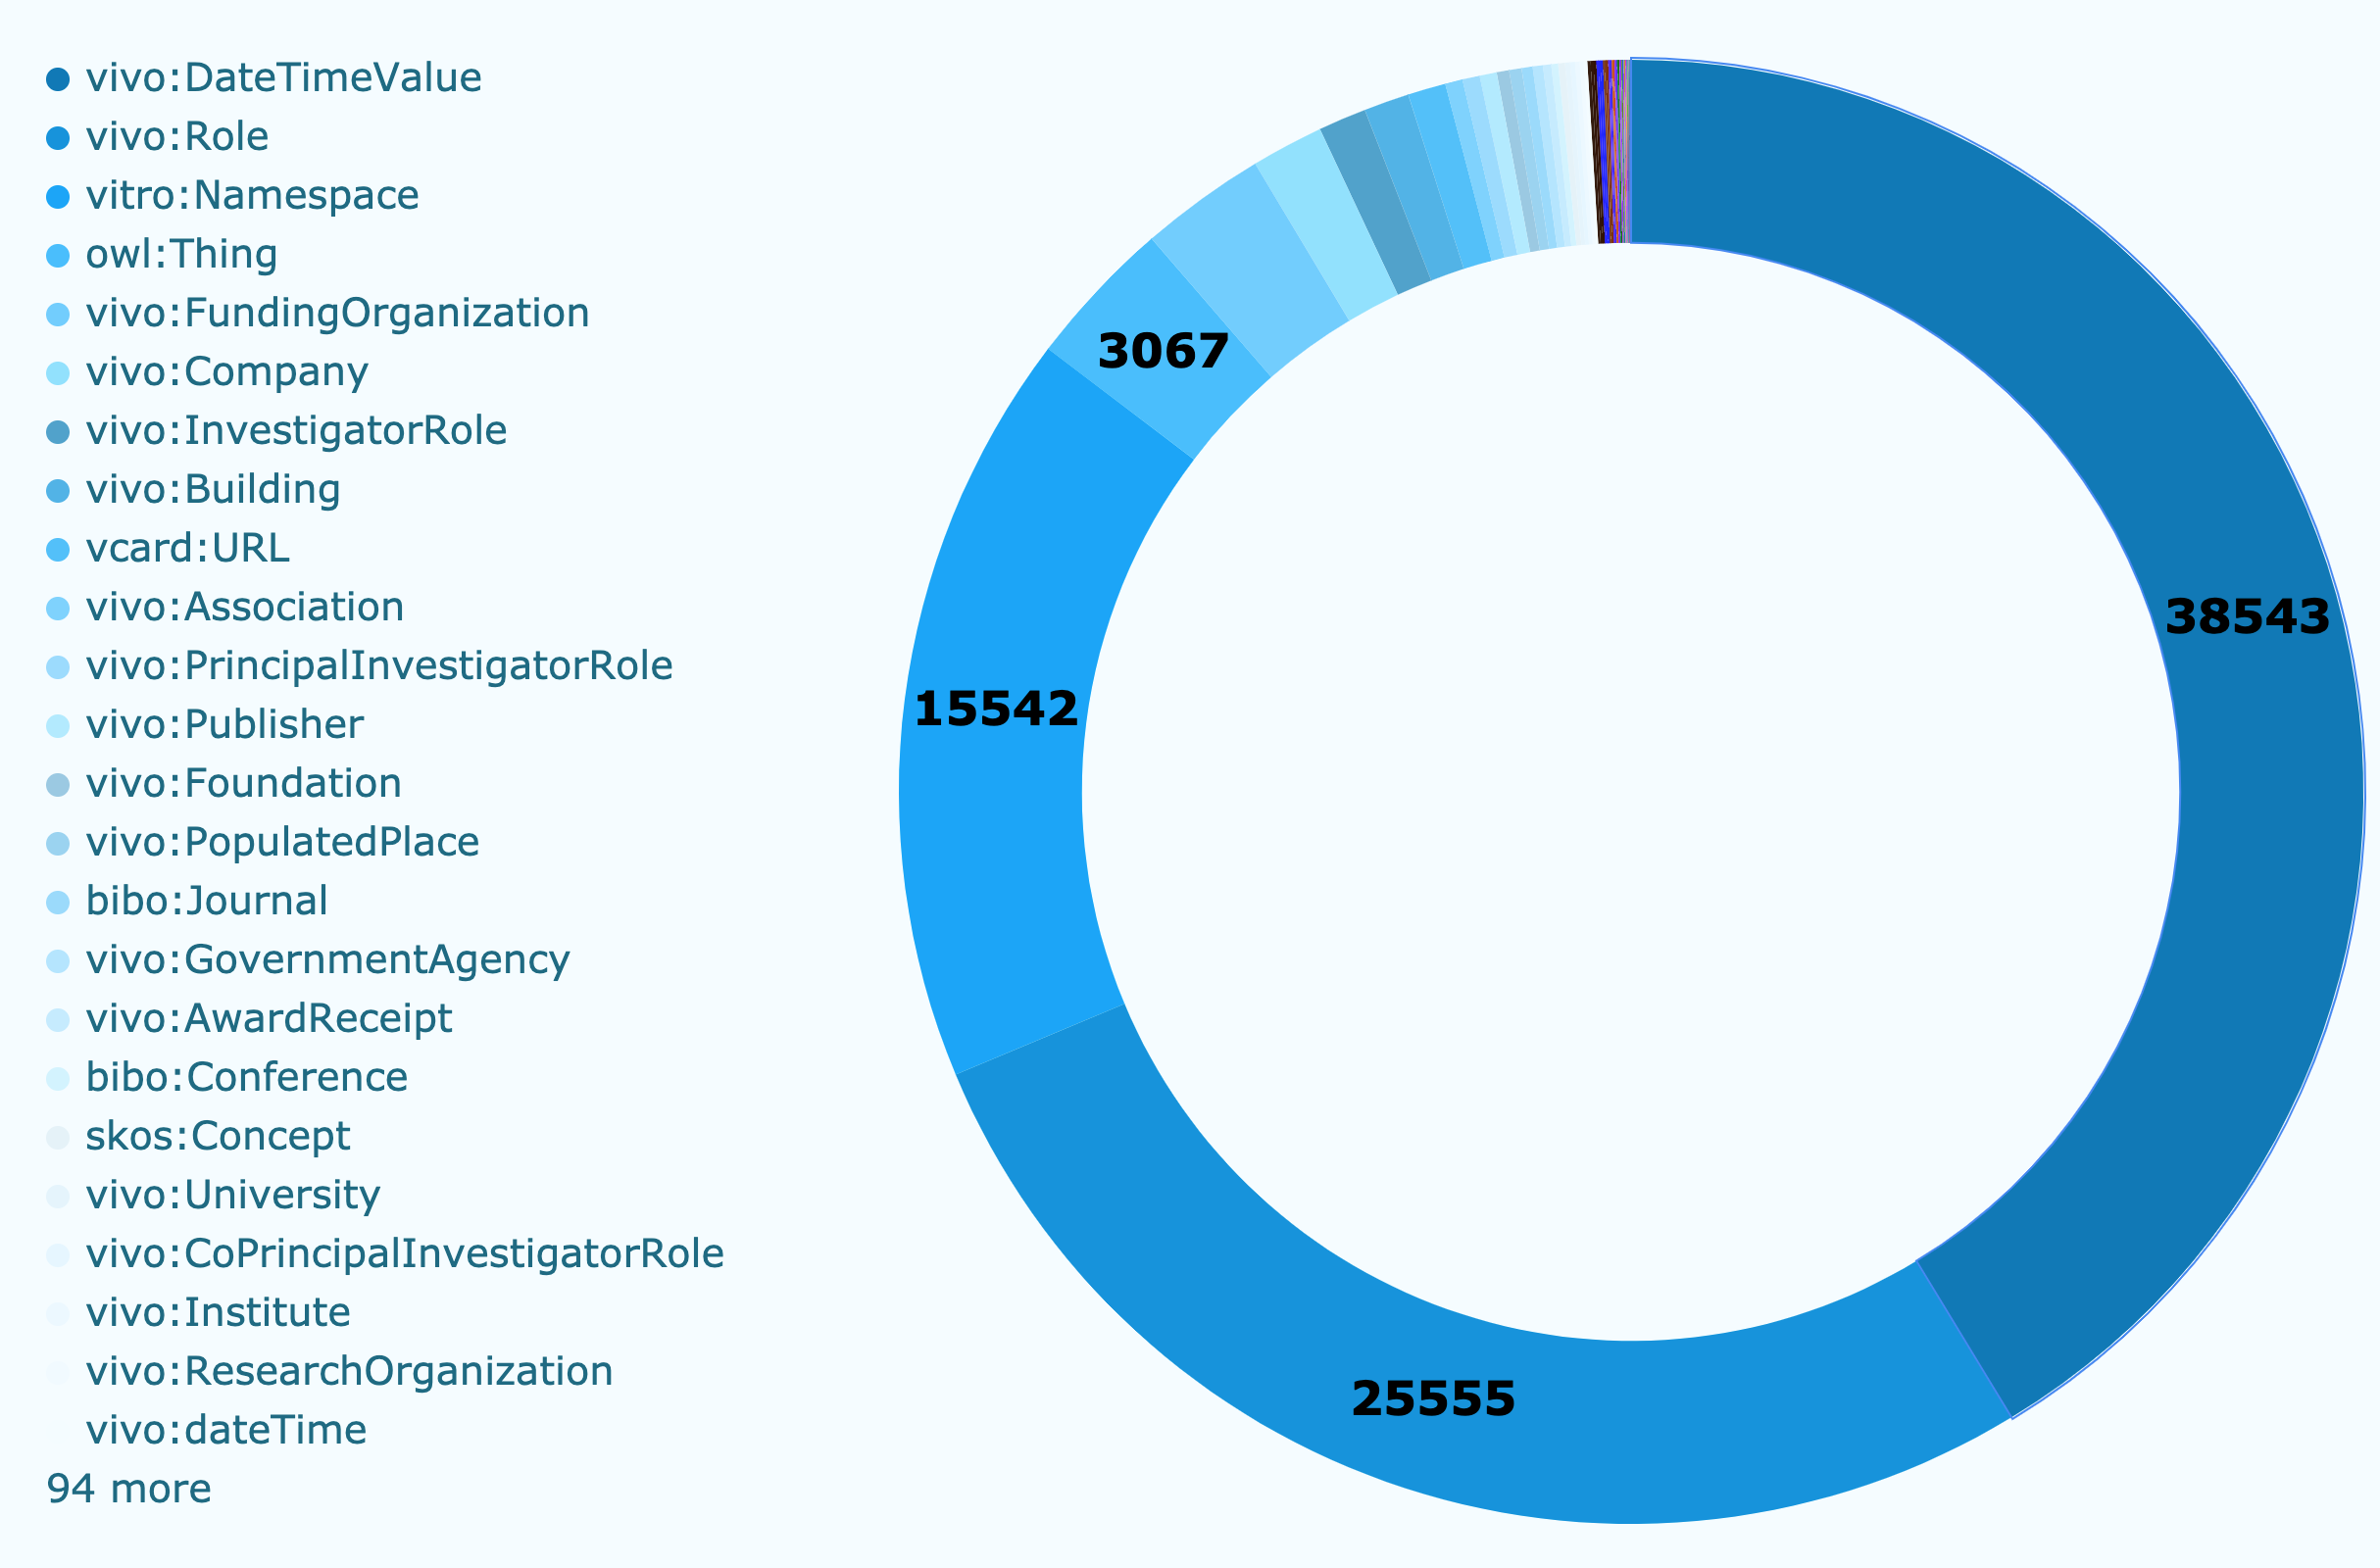
\includegraphics[width=\textwidth]{orphan-types.png}
\caption{Naively orphaned nodes by type. There were over 100 different types of naively orphaned nodes -- these are only the top 35 most frequent occurrences. (Using "most specific" type(s), no superclasses.)}
\label{fig:output}
\end{figure}

\subsubsection*{Connected Components}
This approach yielded interesting information about the global topology of the graph, but it was less effective at uncovering orphans. We calculated the connected components under three sets of constraints. First, we considered every node in the graph with a URI that corresponded to a VIVO entity (using a regex). The results of the algorithm are shown in Figure 3. The graph consists of one large connected component and many tiny connected islands. Then, we re-ran the algorithm but discarded nodes of "metadata" types: "vivo:Concept" and "vivo:Organization". The results are shown in Figure 4. This subgraph still consisted mainly of one large connected component. Finally, we re-ran the algorithm and discarded nodes with a degree of over 100. We wanted to determine whether the graph was "robustly" connected or was connected due to a few "supernodes" that hold the graph together. The results are shown in Figure 5. The graph still had a very large connected component.

\begin{figure}[h!]
\centering
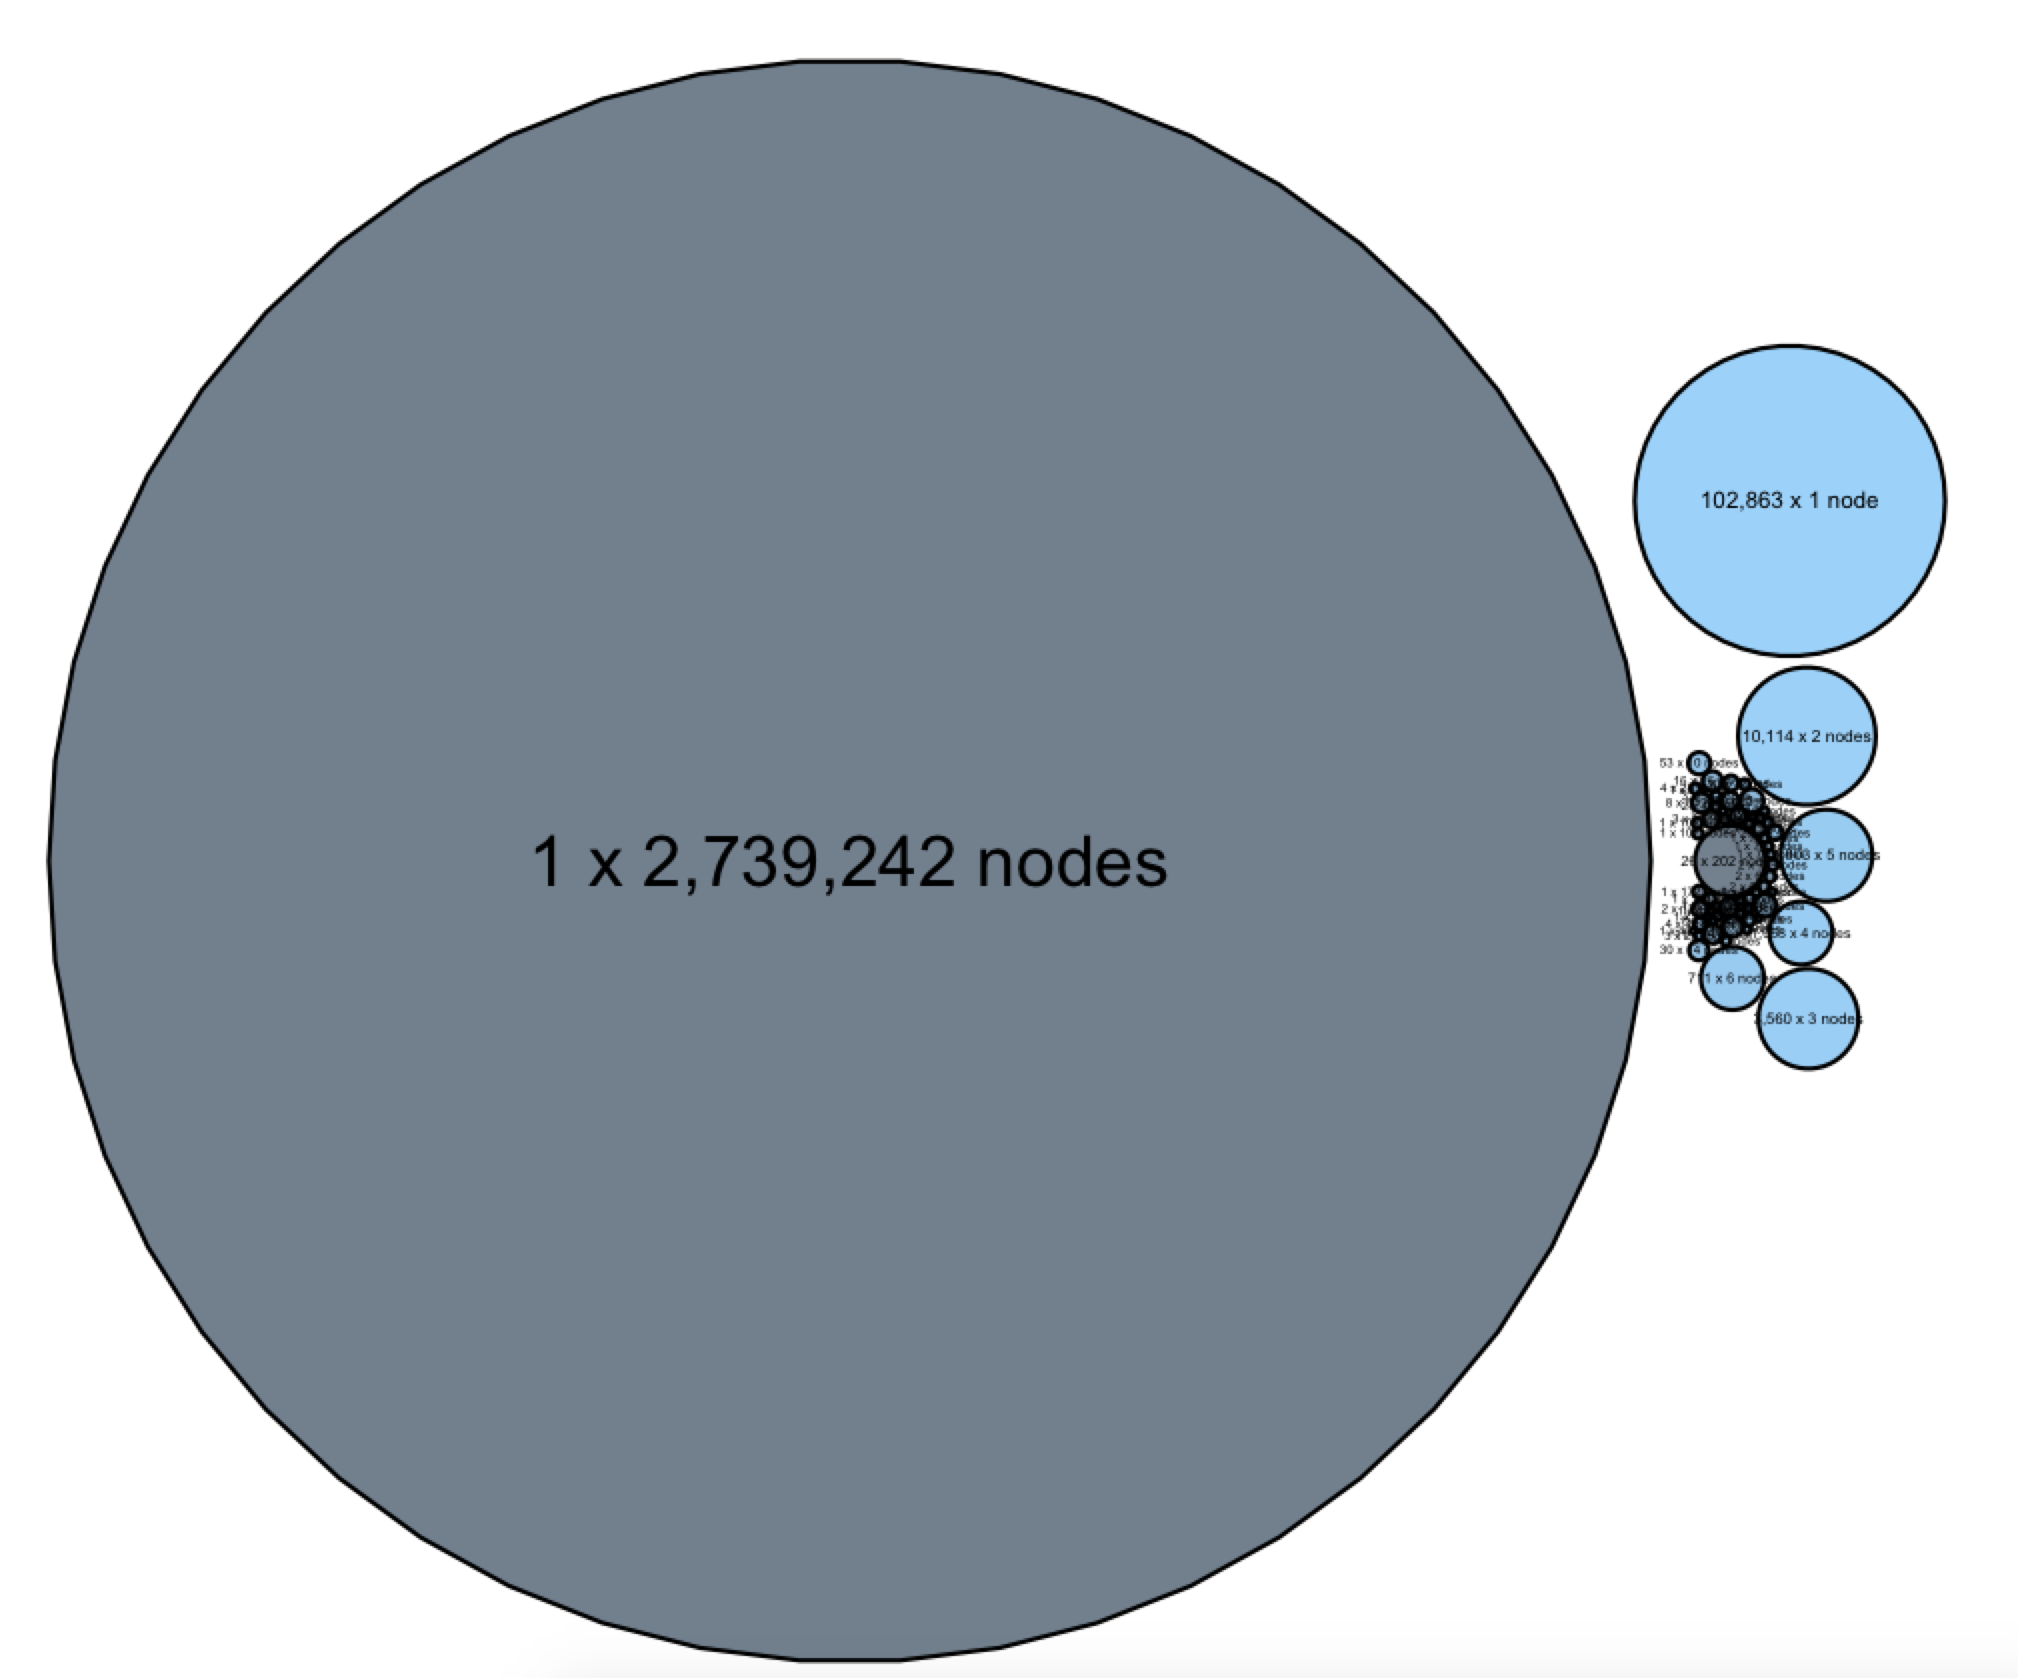
\includegraphics[width=8cm]{cc-actual.png}
\caption{Connected Components of UF VIVO (area proportional to size)}
\label{fig:output}
\end{figure}

\begin{figure}[h!]
\centering
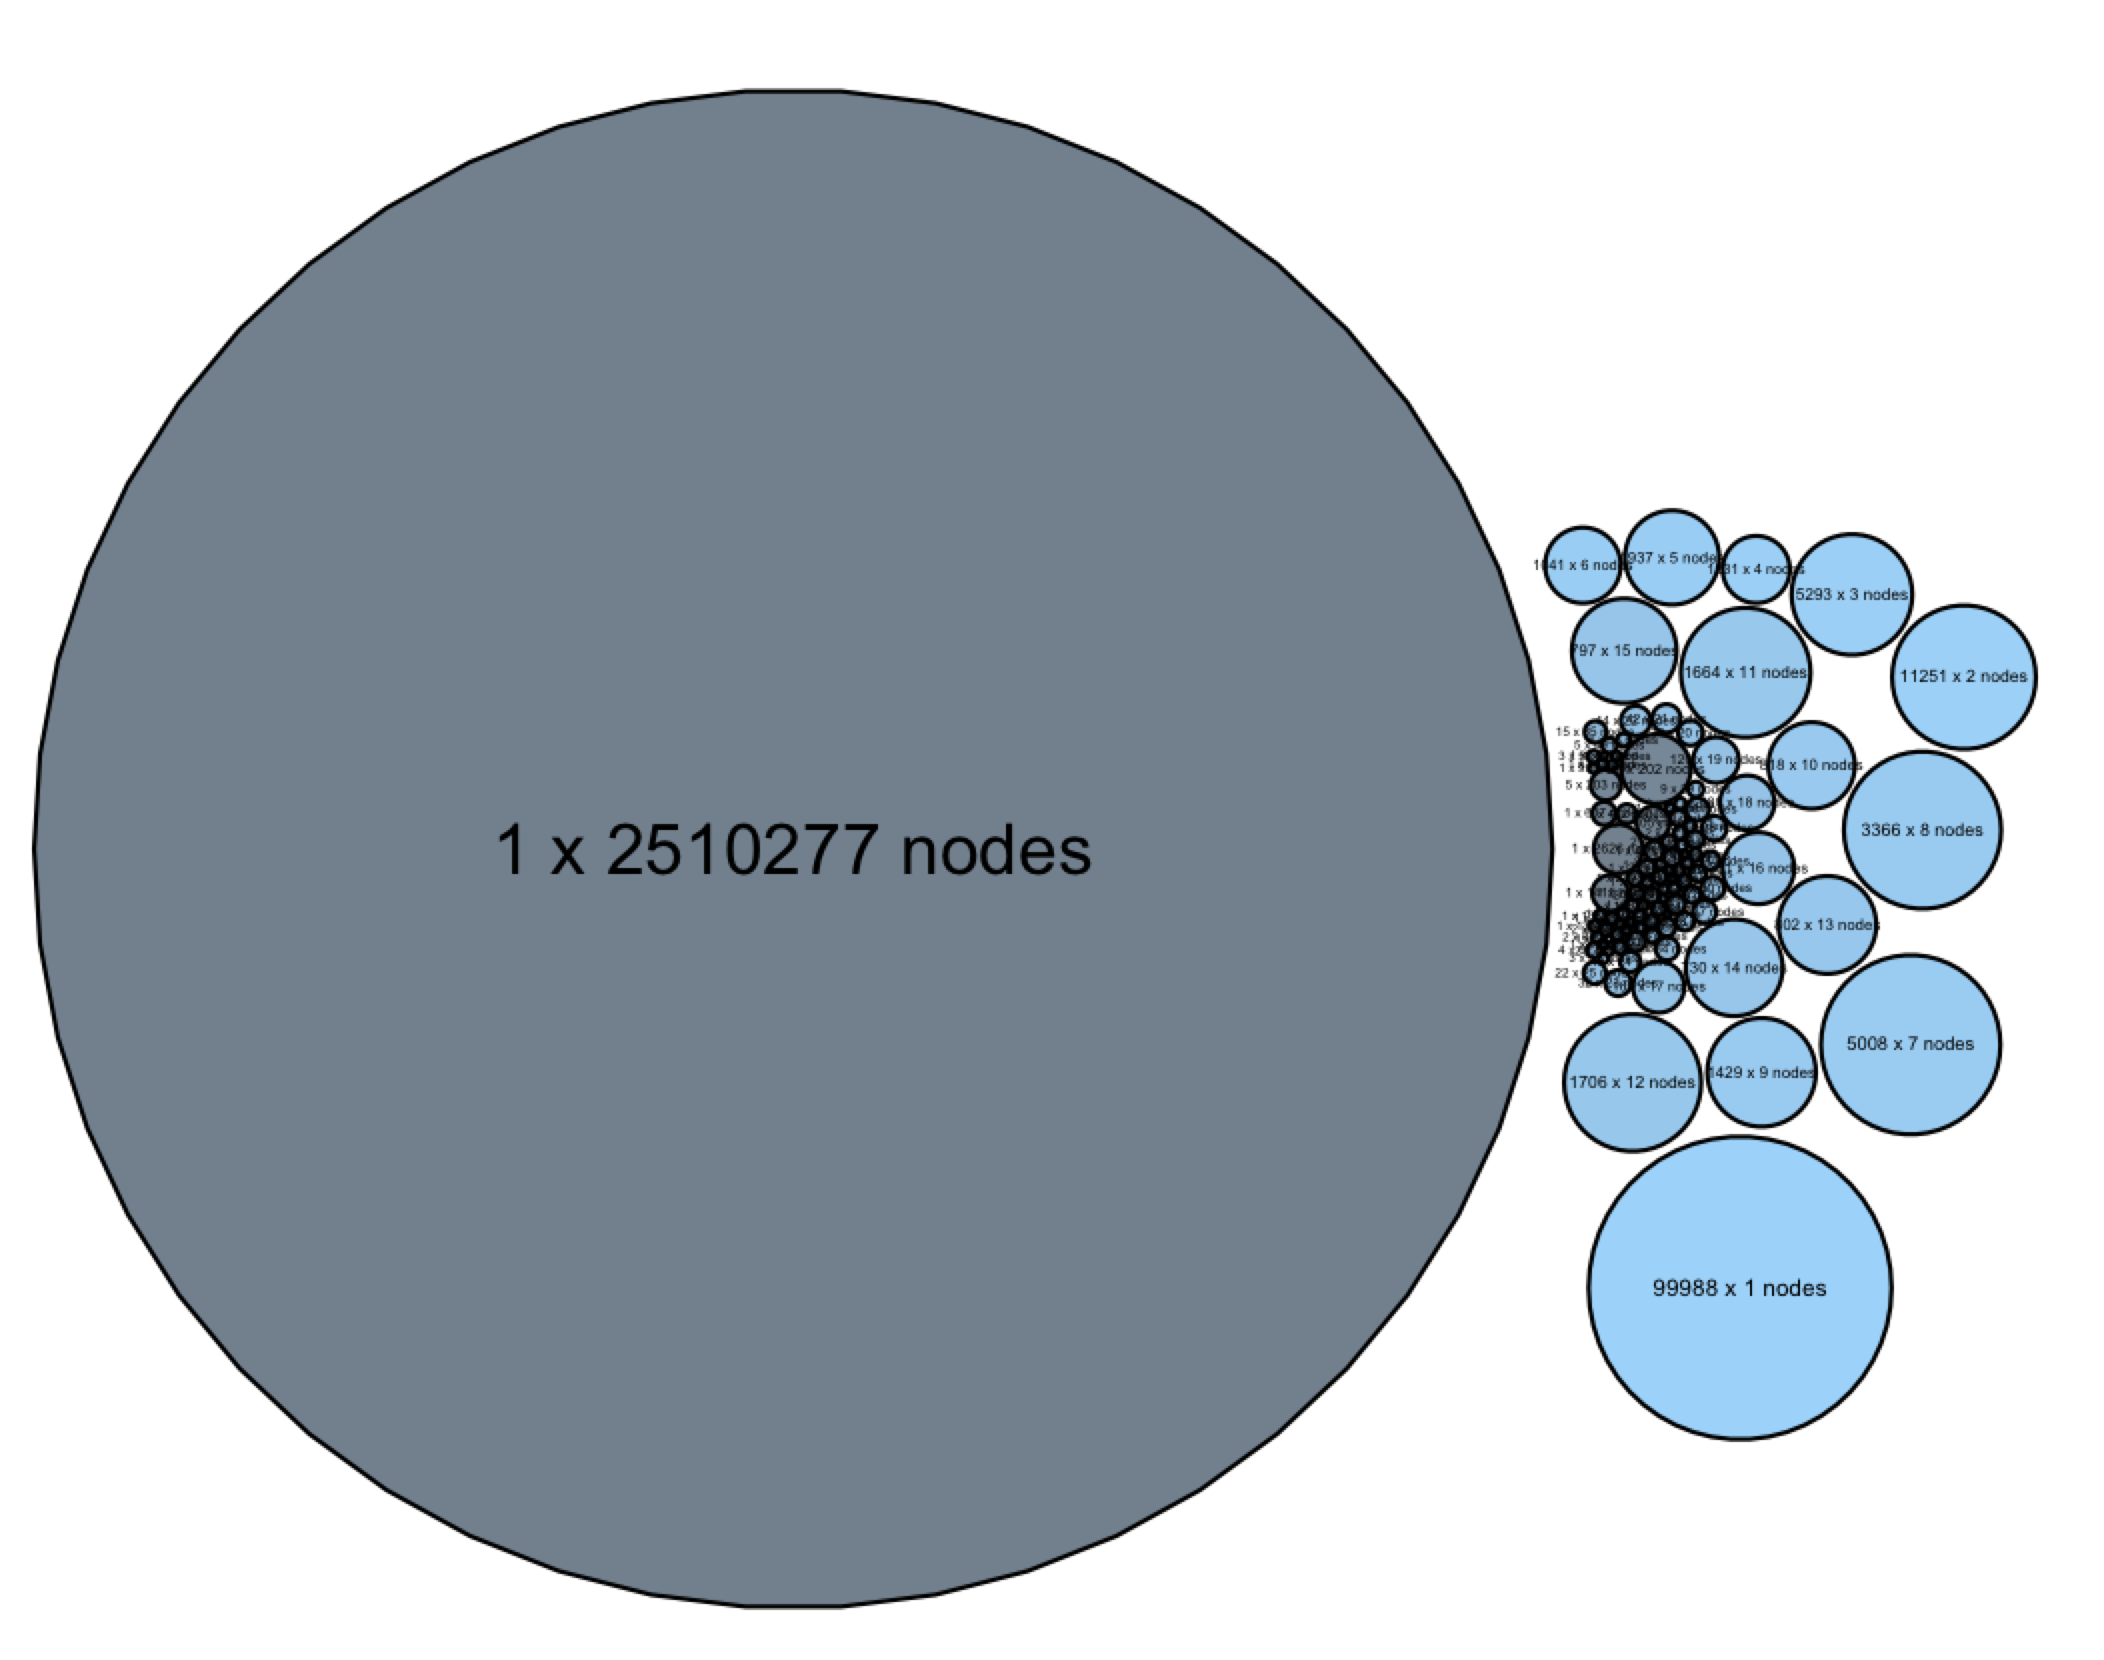
\includegraphics[width=8cm]{cc-2.png}
\caption{Connected Components of UF VIVO, discarding nodes of type "vivo:Organization" or "vivo:Concept" (area proportional to size)}
\label{fig:output}
\end{figure}

\begin{figure}[h!]
\centering
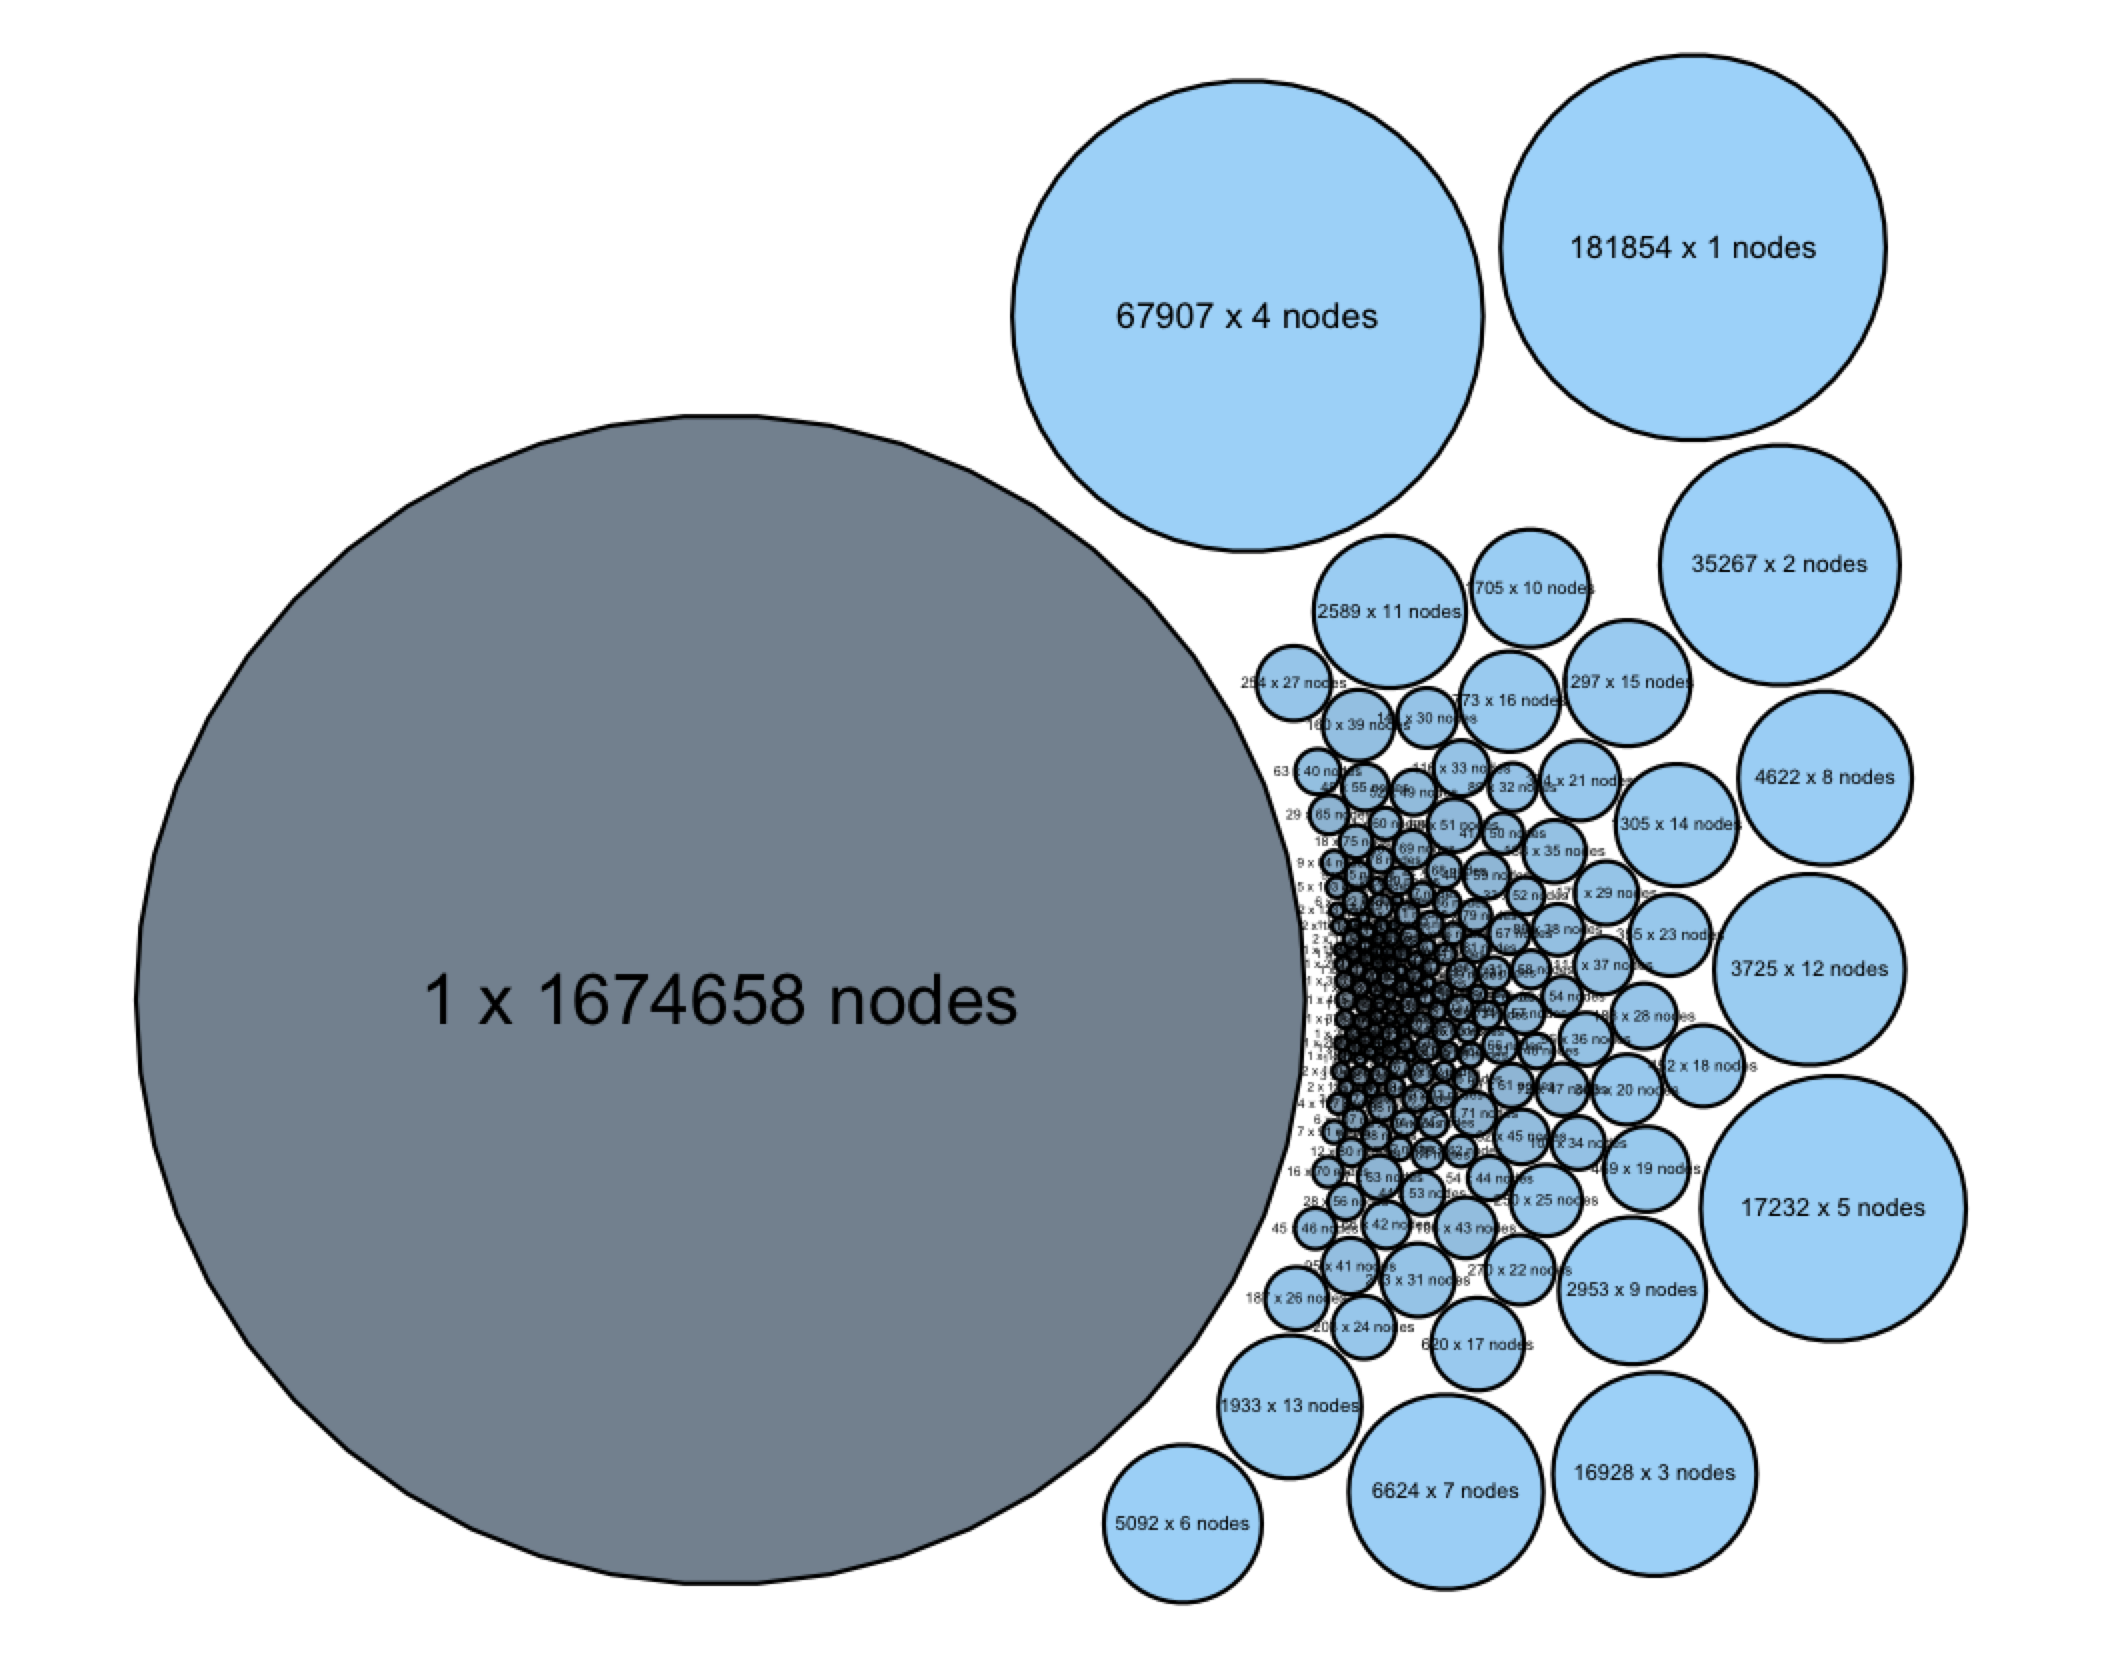
\includegraphics[width=8cm]{cc-3.png}
\caption{Connected Components of UF VIVO, discarding nodes with degree > 100 (area proportional to size)}
\label{fig:output}
\end{figure}

We then analyzed some of the "islands" to determine if they are orphaned. We had already examined the components of size 1 in the previous approach, so we examined some higher-order components. The first approach was creating a type histogram. (Since nodes can have multiple types, we created our histogram using the set of all the node's types.) As shown in Figure 6, many of the low-degree islands also share the exact same types.

\begin{figure}[h!]
\centering
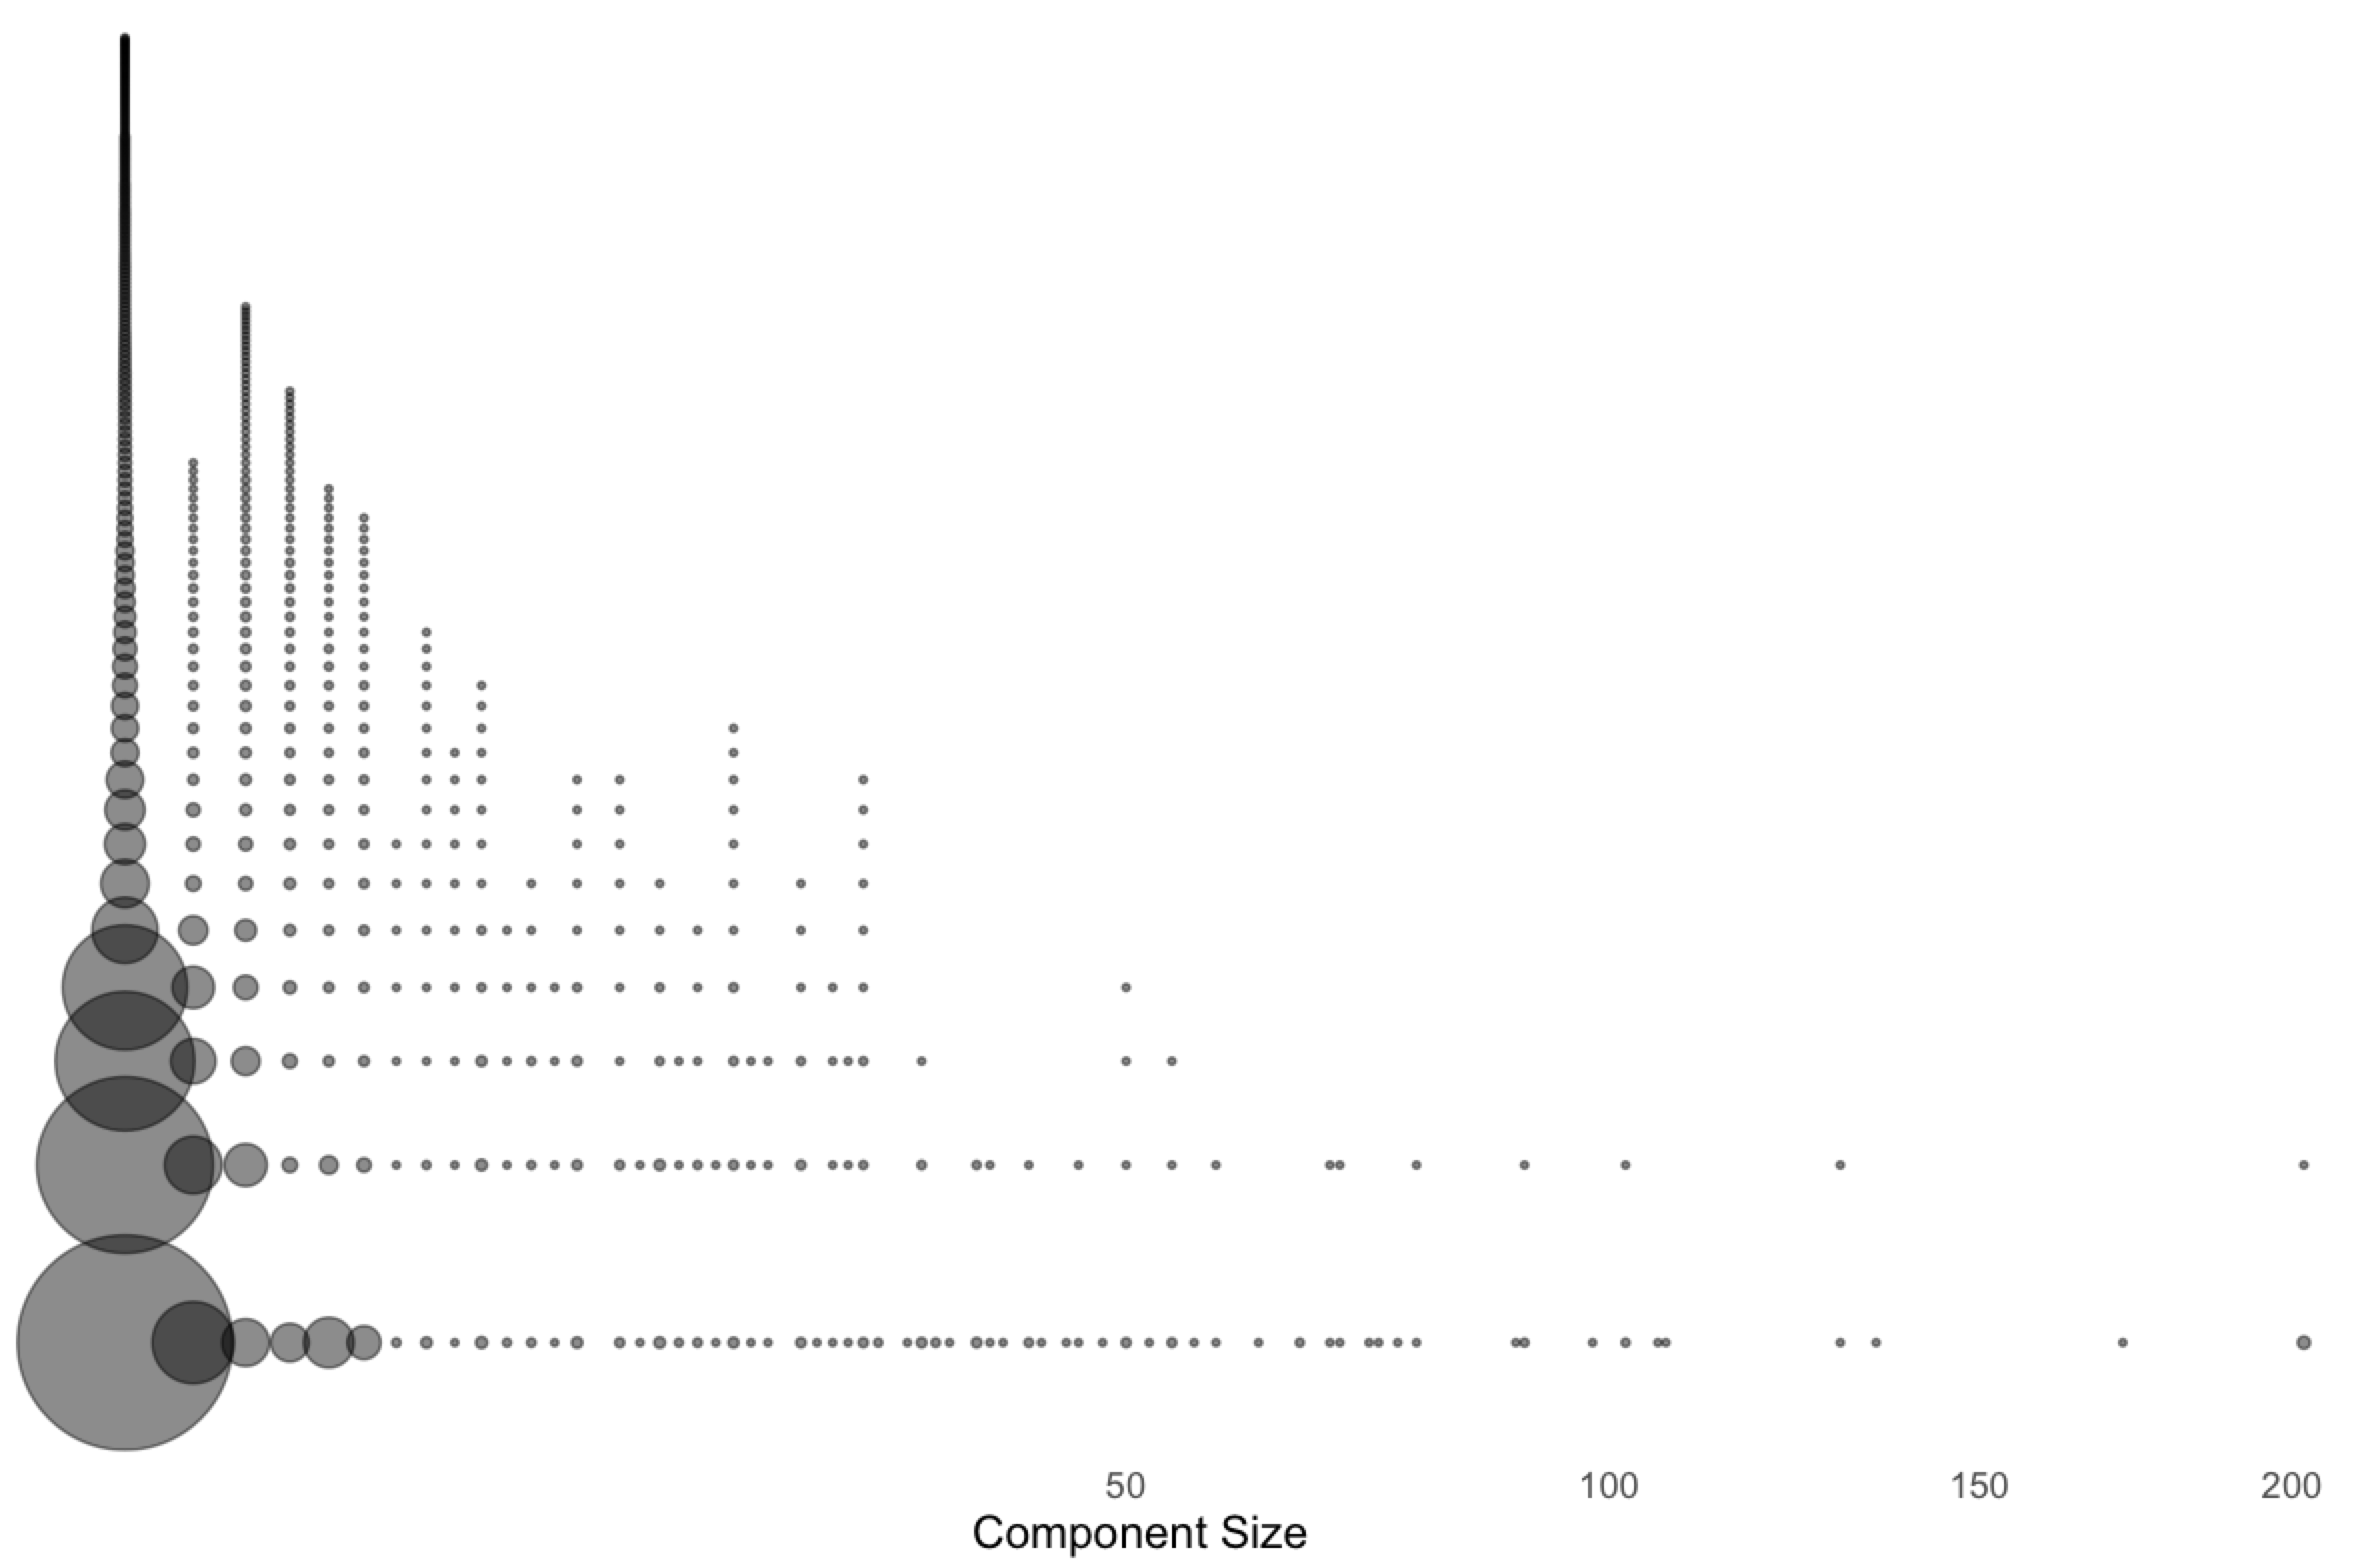
\includegraphics[width=\textwidth]{type-histogram.png}
\caption{Histogram of the distinct type composition of the connected components. Each circle corresponds to a type composition, and its area is proportional to the number of occurrences of that composition.}
\label{fig:output}
\end{figure}

\pagebreak

Finally, after we examined a few sample islands, we determined that few conclusions could be drawn about validity. For example, \url{http://vivo.ufl.edu/individual/n0190888667} is in a component of size 5 (person + vcard + 3 attributes). However, the component describes Magalie Bruneus, an actual UF faculty member with no activity in VIVO. As another example, \url{http://vivo.ufl.edu/individual/n1753230437} is in a connected component of size 13. However, this is a valid paper written by real people, as shown in Figure 7.

\begin{figure}[h!]
\centering

\includegraphics[width=6cm]{valid-paper.png}
\caption{This is a perfectly-valid paper in its own connected component of size 13.}
\label{fig:output}
\end{figure}

\pagebreak
\subsubsection*{Constraint-Checking}
This approach yielded around 10,000 violations of the VIVO ontology and schema [VIVO], listed in Figure 8. We will discuss some of the larger classes of orphans. First, we found 5,000 orphaned vcards -- more specifically, "vcard:Individual"s without an entity that it is "obo:contactInfoFor". This problem has already been noted by CTS-IT. Additionally, we found 3,000 people without vcards -- in other words, "foaf:Person"s without "vcard:Individual"s as "obo:contactInfoFor". However, we noticed that many of these entities were dummy entities created to satisfy generic roles, like "Director" and "Staff". We also found 230 "vivo:AwardReceipt"s without "foaf:Agents" who received the award, and found that nearly all of the 10,000 "vivo:AwardReceipt"s did not correspond to a "vivo:Award", which violates the VIVO ontology. However, not all of these issues may need to be corrected, since the VIVO application may be using these fields for different or internal purposes.

\begin{figure}[h!]
\centering
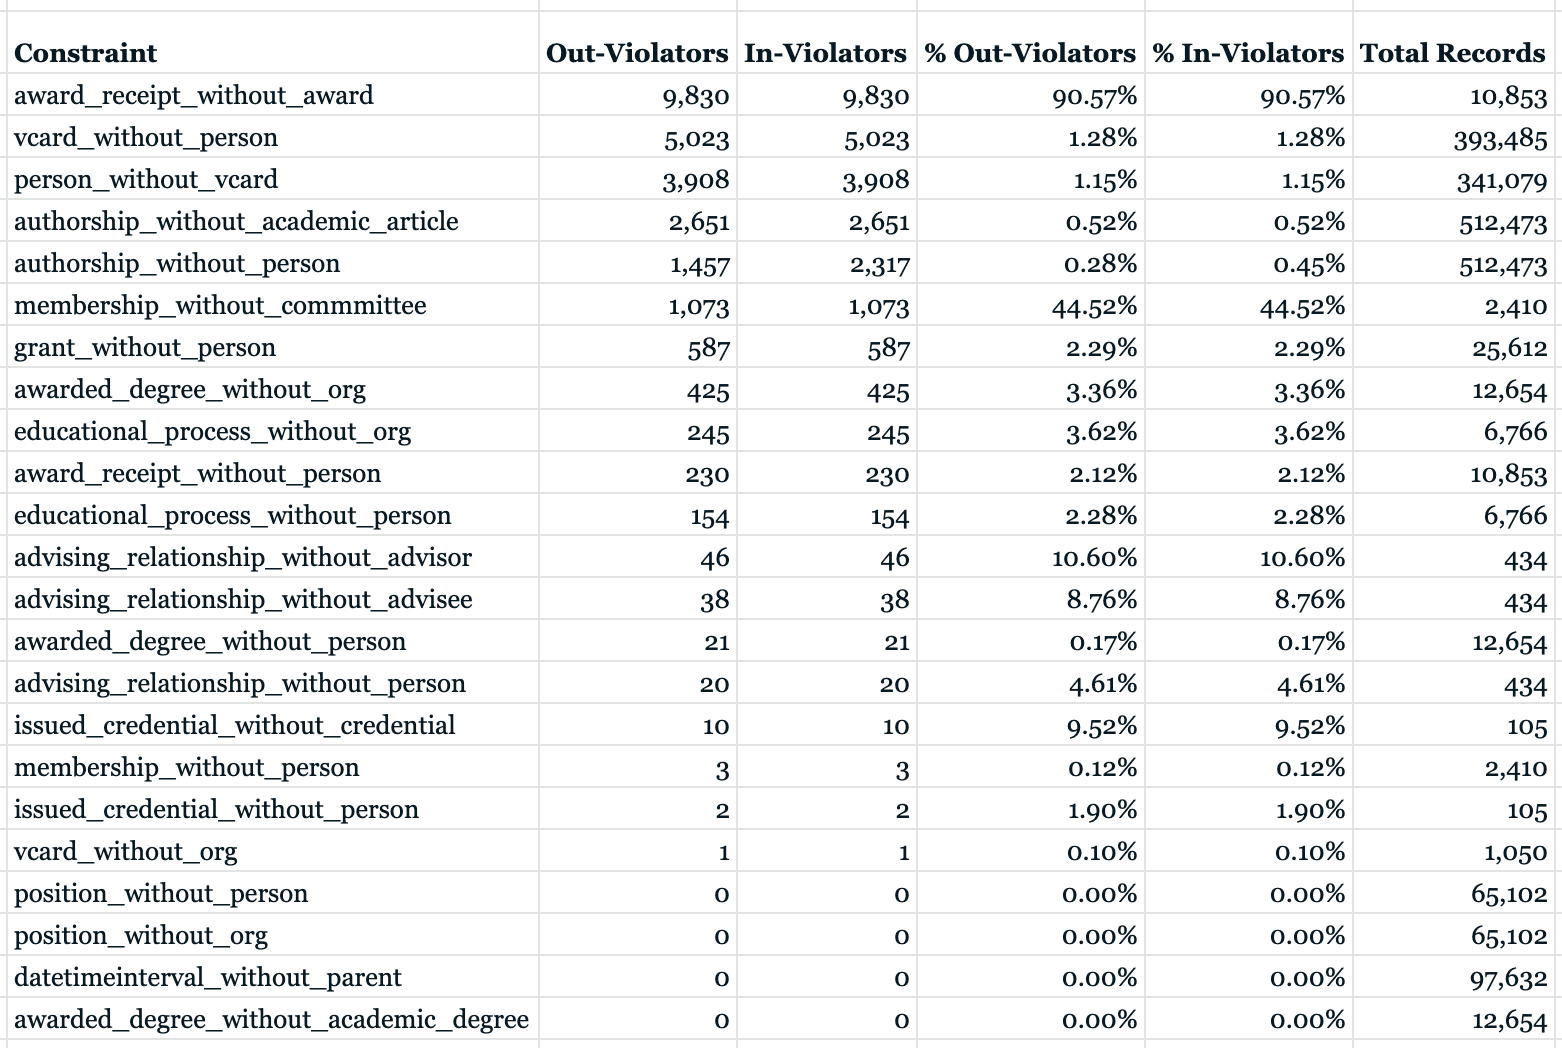
\includegraphics[width=\textwidth]{violators.png}
\caption{Constraints checked. VIVO is a directed graph, but most edges are expected to exist in both directions, so we define an "out-violator" as a node without a correct outward edge. Notice that the constraint "authorship\_without\_person" had more in-violators than out-violators.}
\label{fig:output}
\end{figure}

\subsubsection*{Other Orphaning}
We found several small discrepancies during the analysis, and we will discuss them in this section. First, there are some individuals with extremely long names, due to parsing issues. For example, \url{http://vivo.ufl.edu/individual/n5523339036} has a name over 1,000 characters long -- it is a ';'-separated list of around 100 names. This problem has already been corrected by CTS-IT.

We also found that the entity \url{http://vivo.ufl.edu/individual/n130884} that is both a "foaf:Organization" and a "vcard:Organization", which is not correct.

We also found an entity \url{http://vivo.ufl.edu/individual/n81500} that is a "vivo:File" without a download location.

Finally, we also found that some entities had URIs that were not single URIs but a ';'-separated list of URIs (i.e., "<uri;uri;uri...>"). We could not verify in [NQuads] or [RDF] how these were to be interpreted. One example is \url{http://vivo.ufl.edu/individual/n659903787;http://vivo.ufl.edu/individual/n81818;http://vivo.ufl.edu/individual/n9307328350;http://vivo.ufl.edu/individual/n68632821}. This specific entity is associated with a list of authors for the paper \url{http://vivo.ufl.edu/individual/n8110013759}. It is clear that the VIVO application does not appear to be interpreting it correctly, as \url{http://vivo.ufl.edu/individual/n81818} (Wang, Min) is not listed as an author of the paper.

\section*{Conclusions}
In this project, we examined data quality in the UF VIVO graph database. Although the overall quality of UF VIVO's 30M+ triples is quite good, we discovered tens of thousands of orphans and constraint violations, and we determined that many of these can immediately be removed from the database. Additionally, we analyzed the global topology of the VIVO graph and determined that it is healthy and robustly connected. The code used for the analysis, as well as additional documentation, is available at \url{https://github.com/garyg1/cis4914-sp20}. We were not able to determine the root cause of some of the orphaning; this is partially due to the author's extended illness during March and April. However, this task may be impossible, due to the volume of orphaned data and the potential non-availability of logs. Future work would include an additional validation of the orphans found against the current UF VIVO (instead of a snapshot), followed by deleting the orphaned records.

\section*{Standards}
All programming was done in Python 3.7 according to the Python Language Reference [Python], and all code was executed in a Python 3.7.6 runtime on macOS.

\section*{Constraints}
All code had to be executed on the available equipment: a 2015 MacBook Pro with 8GB of RAM and 128GB of disk space. 

% \begin{lstlisting}
% a := 1;
% \end{lstlisting}
% 
% \begin{figure}[h!]
% \centering
% 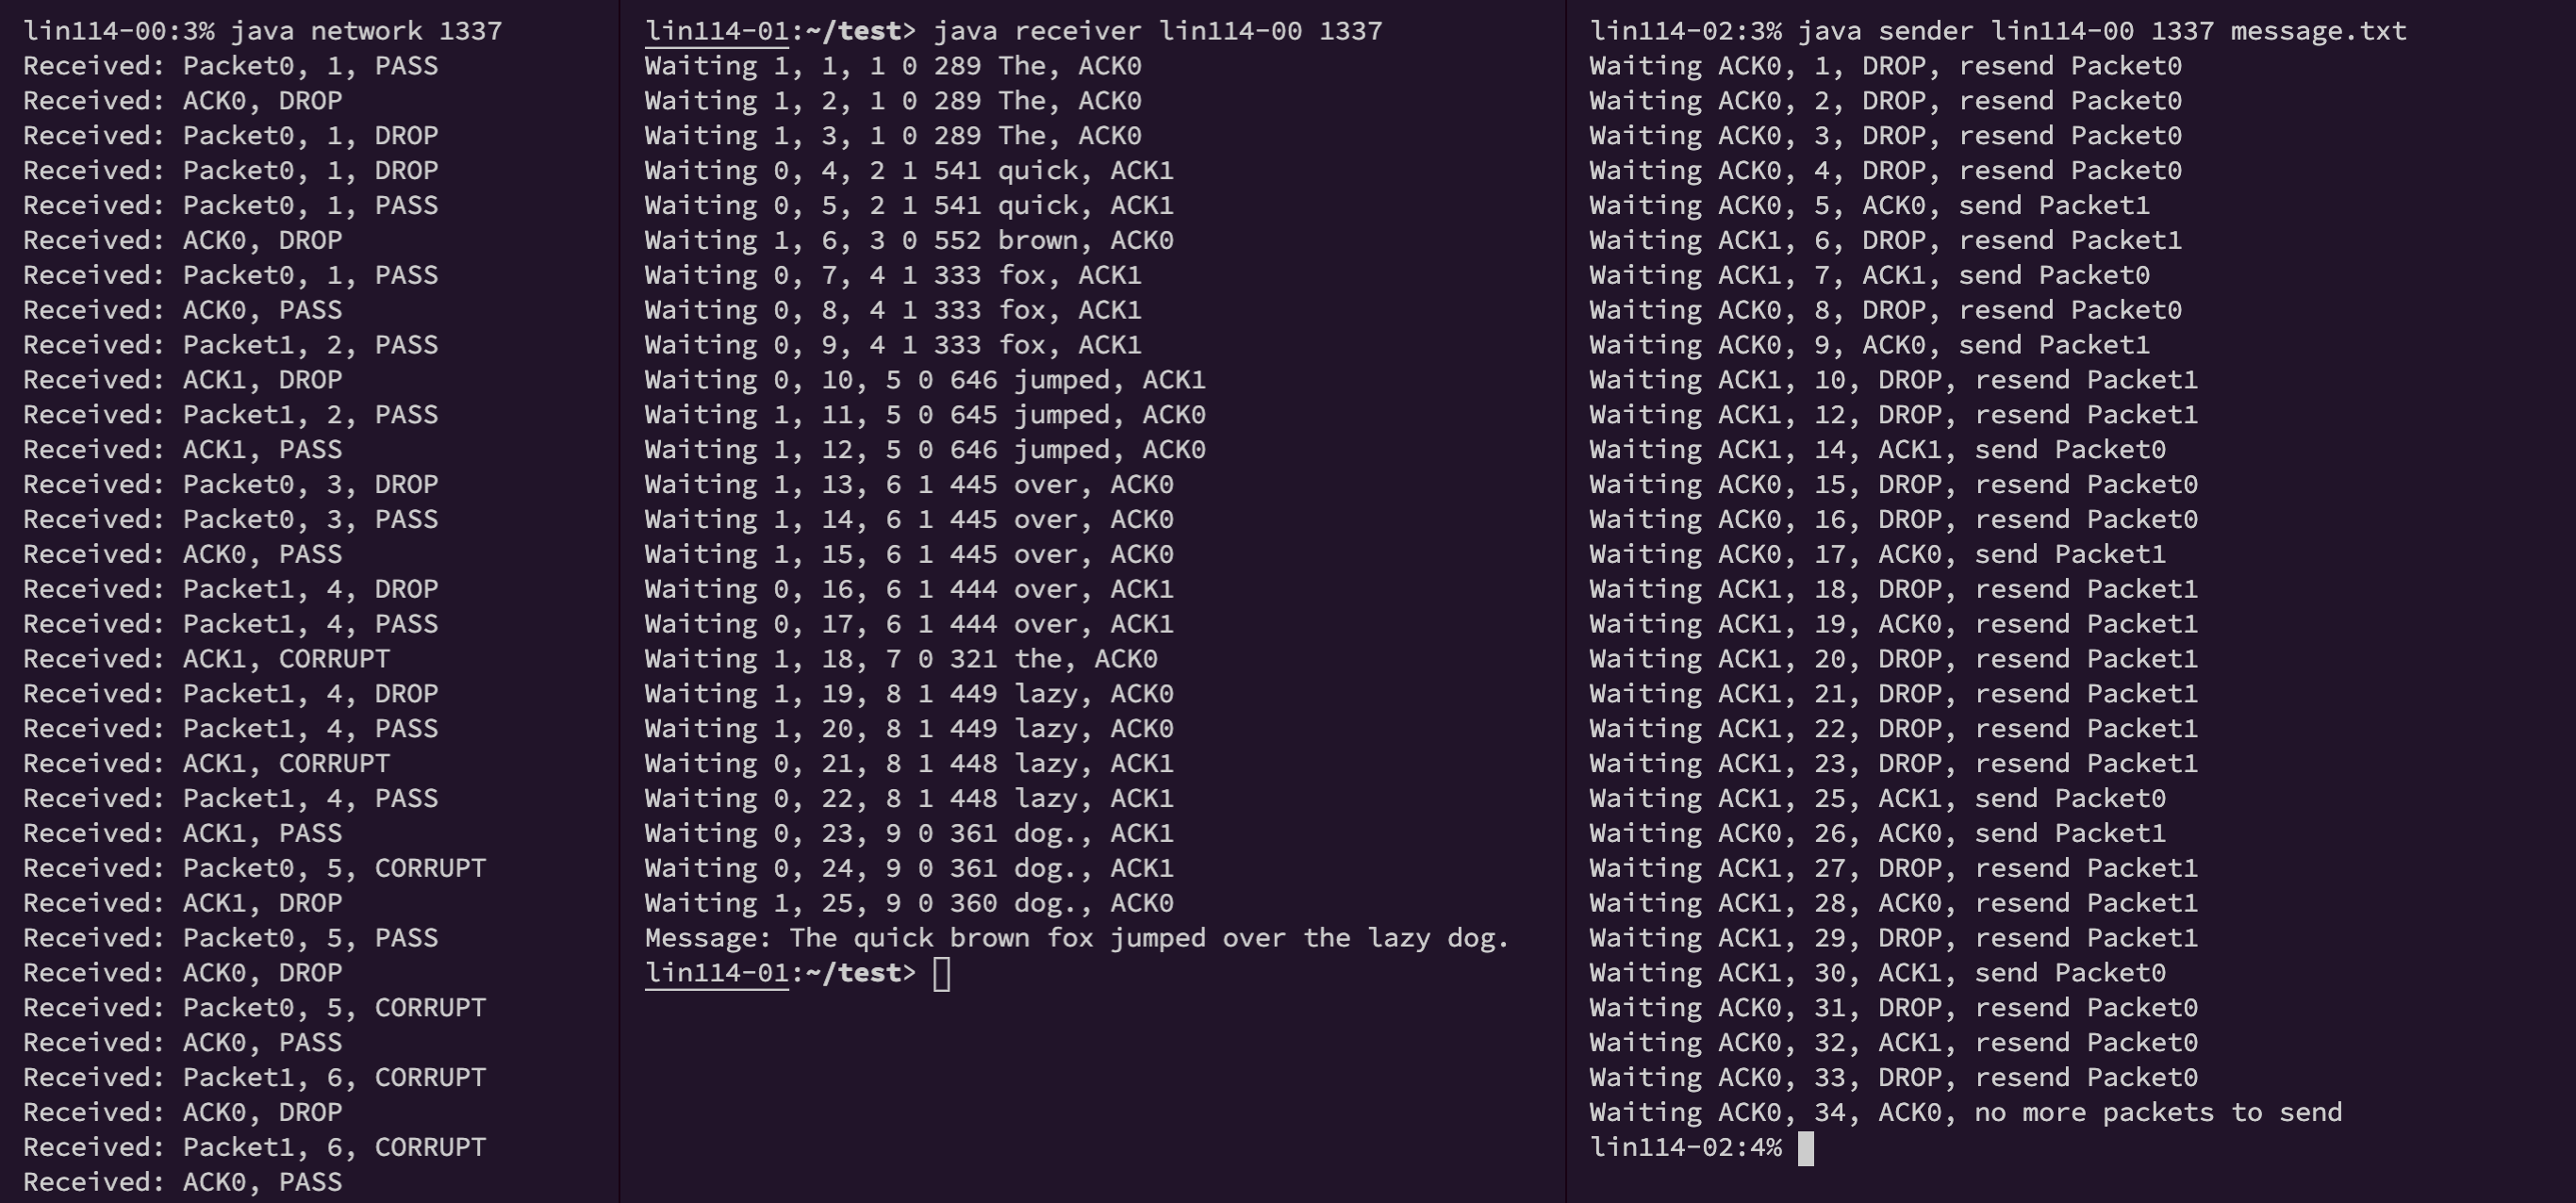
\includegraphics[width=\textwidth]{output.png}
% \caption{An example execution.}
% \label{fig:output}
% \end{figure}

\section*{Acknowledgments}
The author thanks Christopher Barnes for advising the project, and the UF CTS-IT for providing access to the VIVO data. The author also thanks Taeber Rapczak for his excellent help and guidance.

\section*{References}

[NQuads] Gavin Carothers and Lex Machina, Inc. “RDF 1.1 N-Quads: A line-based syntax for RDF datasets”, \url{https://www.w3.org/TR/n-quads/}, W3C (as-of 6 April 2020).

[OWL] Mike Dean, et al. "OWL Web Ontology Language", \url{https://www.w3.org/TR/owl-ref/}, W3C (as-of 15 April 2020).

[Python] Guido van Rossum. “The Python Programming Language”, \url{https://python.org}, Python Software Foundation (as-of 6 April 2020).

[RCirclePacking] "Circle Packing Customization with R", \url{https://www.r-graph-gallery.com/307-add-space-in-circle-packing.html}, r-graph-gallery.com (as-of 17 April 2020).

[RDF] Ora Lassila and Ralph Swick. “Resource Description Framework (RDF) Model and Syntax Specification”, \url{https://www.w3.org/TR/1999/REC-rdf-syntax-19990222}, W3C (as-of 6 April 2020).

[VIVO] Andrew Woods. "VIVO Ontology Diagrams", \url{https://wiki.lyrasis.org/display/VIVODOC111x/Ontology+Diagrams} (as-of 14 April 2020).

\section*{Biography}
Gary Gurlaskie is an undergraduate student studying Mathematics and Computer Science at the University of Florida. He worked at Ultimate Software (data platform engineering) and Intel (software engineering). He plans to graduate in May 2020, and upon graduation will move to Portland to work at Intel full-time. He has always wanted to have a cat, so he will obtain one when he moves to Oregon.

\end{document}

